\documentclass[./../../paper.tex]{subfiles}
\graphicspath{{\subfix{./../../figures/}}}

\begin{document}

% TODO: Change likelihood to delta
% TODO: Discuss the theoretical limits (value goes from -0.5 to 1) 
% \xixi{Do you think that this belongs to the background, too?}
For this measure, we evaluate the likelihood of a counterfactual trace by determining whether a counterfactual leads to the desired outcome or not. For this purpose, we use the predictive model, which returns a prediction for each counterfactual sequence. As we are predicting process outcomes, we typically predict a class. However, forcing a deterministic model to produce a different class prediction is often difficult. Therefore, we can relax the condition by maximising the prediction score of the desired counterfactual outcome\autocite{molnar2019}. If we compare the difference between the counterfactual prediction score with the factual prediction score, we can determine an increase or decrease. Ideally, we want to increase the likelihood of the desired outcome. We refer to this value as \emph{delta}. However, the binary case introduces some noteworthy considerations. 

Within this task setting, we have to consider multiple cases. First, the prediction score is typically limited to a domain within 0 and 1, which we can interpret as a probability distribution. Hence, if the model score is 0.6, then the model has the confidence of 60\% that the input can be categorised as belonging to class 1. For instance, within a medical process, we could say the model is 75\% confident that the patient can be cured. Conversely, there's a 25\%  confidence that the \gls{instance} belongs to class 0. We can make decisions by using a threshold. Typically, this threshold lies at 50\%. Hence, we determine that a patient can make decisions by using a threshold. Typically this threshold lies at 50\%. \autoref{fig:delta-space} illustrates how this threshold behaves given the factual prediction score. 


\begin{figure}[htbp]
    \centering
    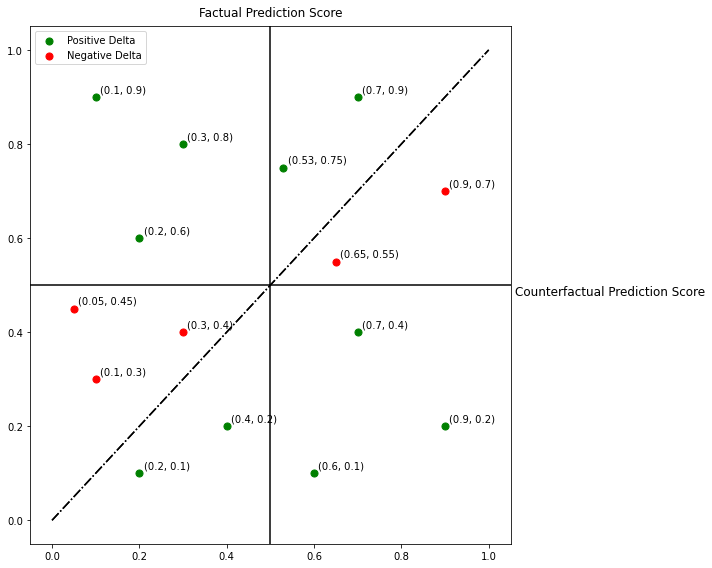
\includegraphics[width=\textwidth]{figures/generated/delta-space.png}
    \caption{An example of which points yield a positive delta given the factual predictions score. Green means the delta is an improvement. Red points signify a negative improvement.}
    \label{fig:delta-space}    
\end{figure}
% n be cured if the model's confidence exceeds 0.5\footnotemark. If we want to determine a soft version of the delta measure, we have to take this decision threshold into account.

We identify 2 cases:
\begin{enumerate}
    \item[Case 1:] A counterfactual generator \emph{flips} the prediction score to the opposite side of the decision threshold. Then, we achieve our general aim, and the difference between the scores directly indicates the counterfactual's success. If we look at \autoref{fig:delta-space}, the two quadrants with only positive delta values cover this case.   
    \item[Case 2:] A counterfactual has the same decision as the factual. For instance, when the counterfactual and factual prediction scores for a patient's recovery chance are below 0.5 or above 0.5. Then, we must consider whether the counterfactual predictions score is moving towards the desired outcome or away from it. 
    \subitem[2.1] If the prediction for the factual decides an outcome of 0, but the predictions score for the counterfactual is even lower, then we did not change the prediction at all. In fact, we increase the chance of the actual factual outcome. That situation is worse than what we desire. For instance, a patient would not want to pursue a counterfactual situation in which his odds of recovery are worse than his current.   
    \subitem[2.2] In contrast, if a prediction model's score leads to an outcome of 0 but the counterfactual returns a higher prediction score than the factual predictions score, a patient might still be interested in the counterfactual. In some situations, even a small improvement is desirable.   
\end{enumerate}

\noindent The sub-cases of case 2 go in both ways. Hence, we have to incorporate each case differently in the delta score. The two quadrants in \autoref{fig:delta-space} that have positive and negative deltas reflect how we interpret these cases.


% \begin{align}
%     \label{eq:likelihood_measure}
%     
% \end{align}


\begin{align}
    \label{eq:delta}
%     d_{a, b}(i, j) & =\min
    delta &= 
    \begin{cases}
            |p(o|s^*)-p(o|s)| &  \text{if }  p(o|s) > 0.5 \text { \& }  p(o|s) > p(o|s^*) \\                 
            -|p(o|s^*)-p(o|s)| &  \text{if }  p(o|s) > 0.5 \text { \& }  p(o|s) < p(o|s^*) \\                 
            |p(o|s^*)-p(o|s)| &  \text{if }  p(o|s) < 0.5 \text { \& }  p(o|s) > p(o|s^*) \\                 
            -|p(o|s^*)-p(o|s)| &  \text{if }  p(o|s) < 0.5 \text { \& }  p(o|s) < p(o|s^*) \\                 
    \end{cases} 
\end{align}

% \begin{align}
%     \label{eq:modified_dl}
%     d_{a, b}(i, j) & =\min
%     \begin{cases}
%         \editDistance{i-1}{j  }+\editCostFunctionNoA & \text { if } i>0                                            \\
%         \editDistance{i  }{j-1}+\editCostFunctionNoB & \text { if } j>0                                            \\
%         \editDistance{i-1}{j-1}+\editCostFunctionBoth & \text { if } i, j>0   \\ & \text { \& } \overline{a}_i=\overline{b}_j                                       \\
%         \editDistance{i-1}{j-1}+ \editCostFunctionNoB +\editCostFunctionNoA  & \text { if } i, j>0  \\ & \text { \& } \overline{a}_i \neq \overline{b}_j                                       \\
%         \editDistance{i-2}{j-2}+\editCostFunction{a_i}{b_{j-1}} + \editCostFunction{a_{i-1}}{b_j} & \text { if } i, j>1 \\ 
%         & \text { \& } \overline{a}_i=\overline{b}_{j-1} \\ 
%         & \text { \& } \overline{a}_{i-1}=\overline{b}_j \\
%         0                                 & \text { \& } i=j=0                                          
%     \end{cases} 
% \end{align}

% TODO: Add plot

% \begin{figure}[htbp]
%     \centering
%     \begin{tikzpicture}[scale=1.5]
%         \tkzInit[xmax=1,ymax=1,xmin=0,ymin=0]
%         \tkzGrid
%         \tkzAxeXY[/tkzdrawX/label=Re,/tkzdrawY/label=Im]
%         \tkzDefPoint(0.5,0.5){A}
%         % \tkzDefPoint(0, sqrt(2)){B}
%         \tkzDefPoint(1,0){B}
%         \tkzDefPoint(0,1){C}
%         \tkzDefPoint(1,1){D}
%         \tkzDefPoint(0,0){E}
%         % \tkzDefCircle[through](A,B)
%         \tkzDrawLine[add= 0.1 and 0,color=blue, dashed](E,D)
%         \tkzDrawLine[add=0 and 0.1, color=blue, dashed](B,C)
%         % \tkzDrawLine[color=green,add=0 and 0](D,C)
%         % \tkzDrawCircle[dashed, color=red](A,B)
%       \end{tikzpicture}
% \end{figure}




% \autoref{eq:likelihood_measure} shows the corresponding formula. 

\footnotetext{Obviously, the domain of the application decides where this threshold lies. One can always argue that confidence of 51\% is close to randomly guessing.}

% \begin{align}
%     \label{eq:likelihood_measure}
%     delta = p(o|s^*)-p(o|s)
% \end{align}

% \noindent Here, $p(o|s)$ describes the probability of an outcome $o$ given a sequence of events $s$. $s^*$ denotes a counterfactual sequence. 

% TODO: Discuss how this formulation favors shorter sequences. It might be solved by using an exact sequence prob computation. Deep-Normalising-Flows with VAE, for instance.
% TODO: Discuss several options here: We can use only likelihood or likelihood improvement. Those are using odds is too aggressive. That difference is bigger. And which to choose. But just using likelihood is similar to feasibility.

\end{document}